%
% teil2.tex -- Beispiel-File für teil2 
%
% (c) 2020 Prof Dr Andreas Müller, Hochschule Rapperswil
%
% !TEX root = ../../buch.tex
% !TEX encoding = UTF-8
%
\section{Inversion 
\label{moebius:section:teil2}}
\kopfrechts{Inversion}
\subsection{Inversion in der komplexen Ebene}

Bei der Inversion wird jeder Punkt \( z \) auf seinen Kehrwert \( \frac{1}{z} \) abgebildet.
Schreibt man
\[
z = r e^{i\varphi}
\]
in Polarform so ergibt sich
\index{Polarform}%
\[
\frac{1}{z} = \frac{1}{r} e^{-i\varphi}.
\]
Dabei gilt:
\begin{itemize}
	\item Der Betrag wird invertiert \( r \rightarrow \frac{1}{r} \).  
	\item Der Winkel wird gespiegelt \( \varphi \rightarrow -\varphi \).
\end{itemize}
Das bedeutet geometrisch:
\begin{itemize}
	\item Punkte nahe bei \(0\) werden weit nach aussen abgebildet. 
	\item Grosse Abstände werden klein.
	\item Kreise können sich stark verformen (werden zu anderen Kreisen oder Geraden).
	\item Der Winkel wird an der reellen Achse gespiegelt.
\end{itemize}
Die folgende Tabelle zeigt, wie sich Kreise und Geraden unter der Inversion verhalten, insbesondere abhängig davon, ob der Punkt \(0\) enthalten ist.



\begin{table}[h]
	\centering
	\begin{tabular}{|c|c|c|}
		\hline
		\textbf{Objekt} & \textbf{Enthält 0?} & \textbf{Ergebnis} \\
		\hline
		Kreis & Ja & Gerade \\
		%\hline
		Kreis & Nein & Kreis \\
		%\hline
		Gerade & Ja & Gerade \\
		%\hline
		Gerade & Nein & Kreis \\
		\hline
	\end{tabular}
\end{table}
\begin{satz}
Kreise, welche den Punkt \(0\) enthalten, werden unter der Inversion auf Geraden abgebildet.
\end{satz}
\begin{proof}
Wir betrachten die allgemeine Kreisgleichung mit Mittelpunkt \(1\) und Radius \(1\)
\[
|z - 1| = 1.
\]
Sei die Inversion gegeben durch
\[
w = \frac{1}{z}
\quad \Leftrightarrow \quad
z = \frac{1}{w}.
\]
Einsetzen von \( z = \frac{1}{w} \) ergibt
\[
\left|\frac{1}{w} - 1\right| = 1.
\]
Nun umformen:
\[
\left|\frac{1 - w}{w}\right| = 1.
\]
Aus den Eigenschaften des Betrags folgt
\[
\frac{|1 - w|}{|w|} = 1.
\]
Multiplikation mit \( |w| \) ergibt
\[
|1 - w| = |w|.
\]
Dies beschreibt eine Gerade, da alle Punkte \( w \) den gleichen Abstand zu den Punkten \(0\) und \(1\) haben.
\end{proof}

\begin{figure}
	\centering
	
	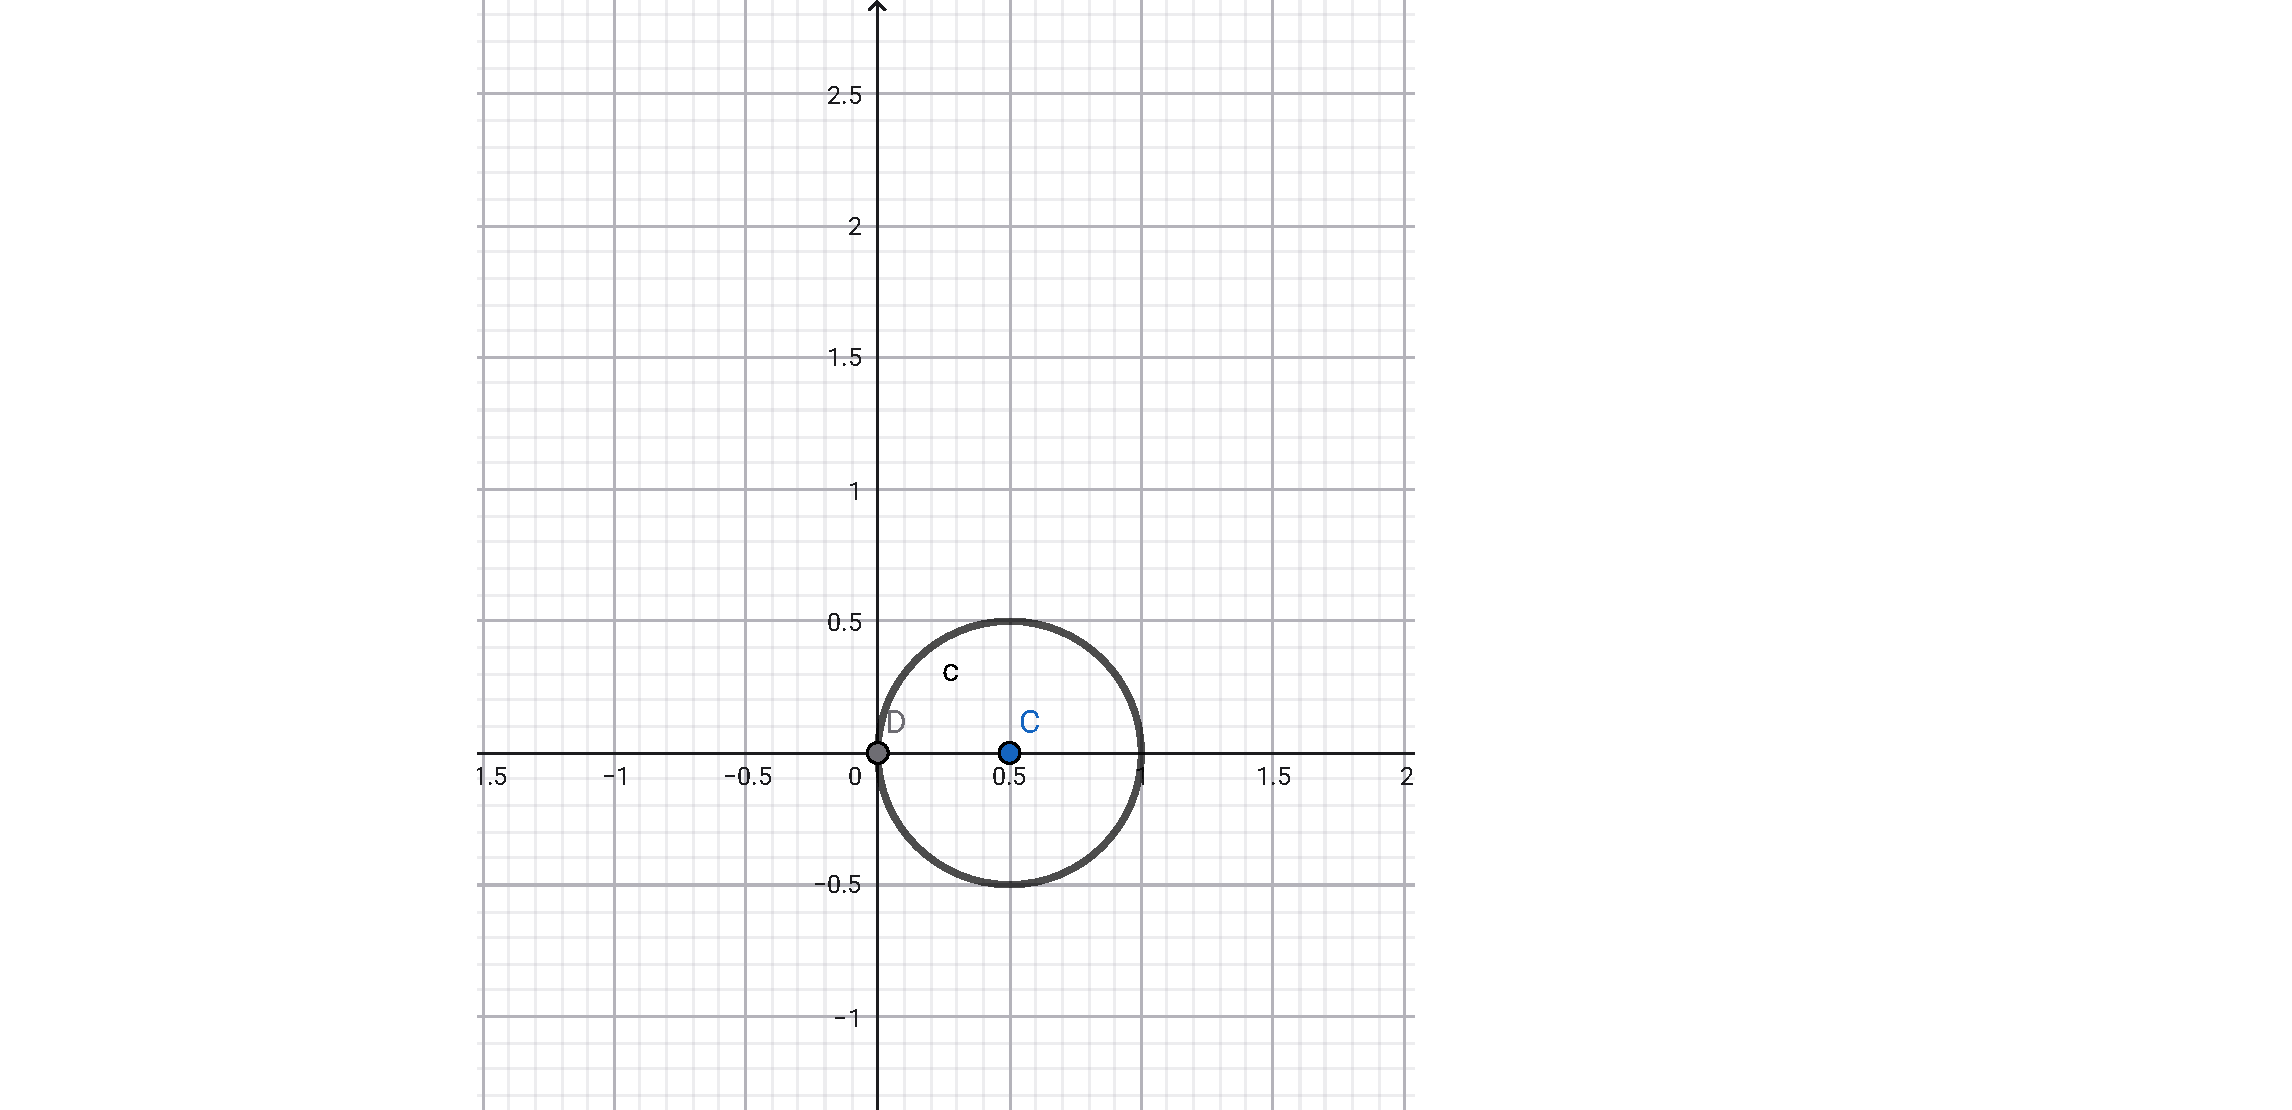
\includegraphics[width=0.6\textwidth]{papers/moebius/bild1.pdf}
	\caption{Vor der Transformation (erstellt mit GeoGebra)}
	
	\vspace{0.8cm}
	
	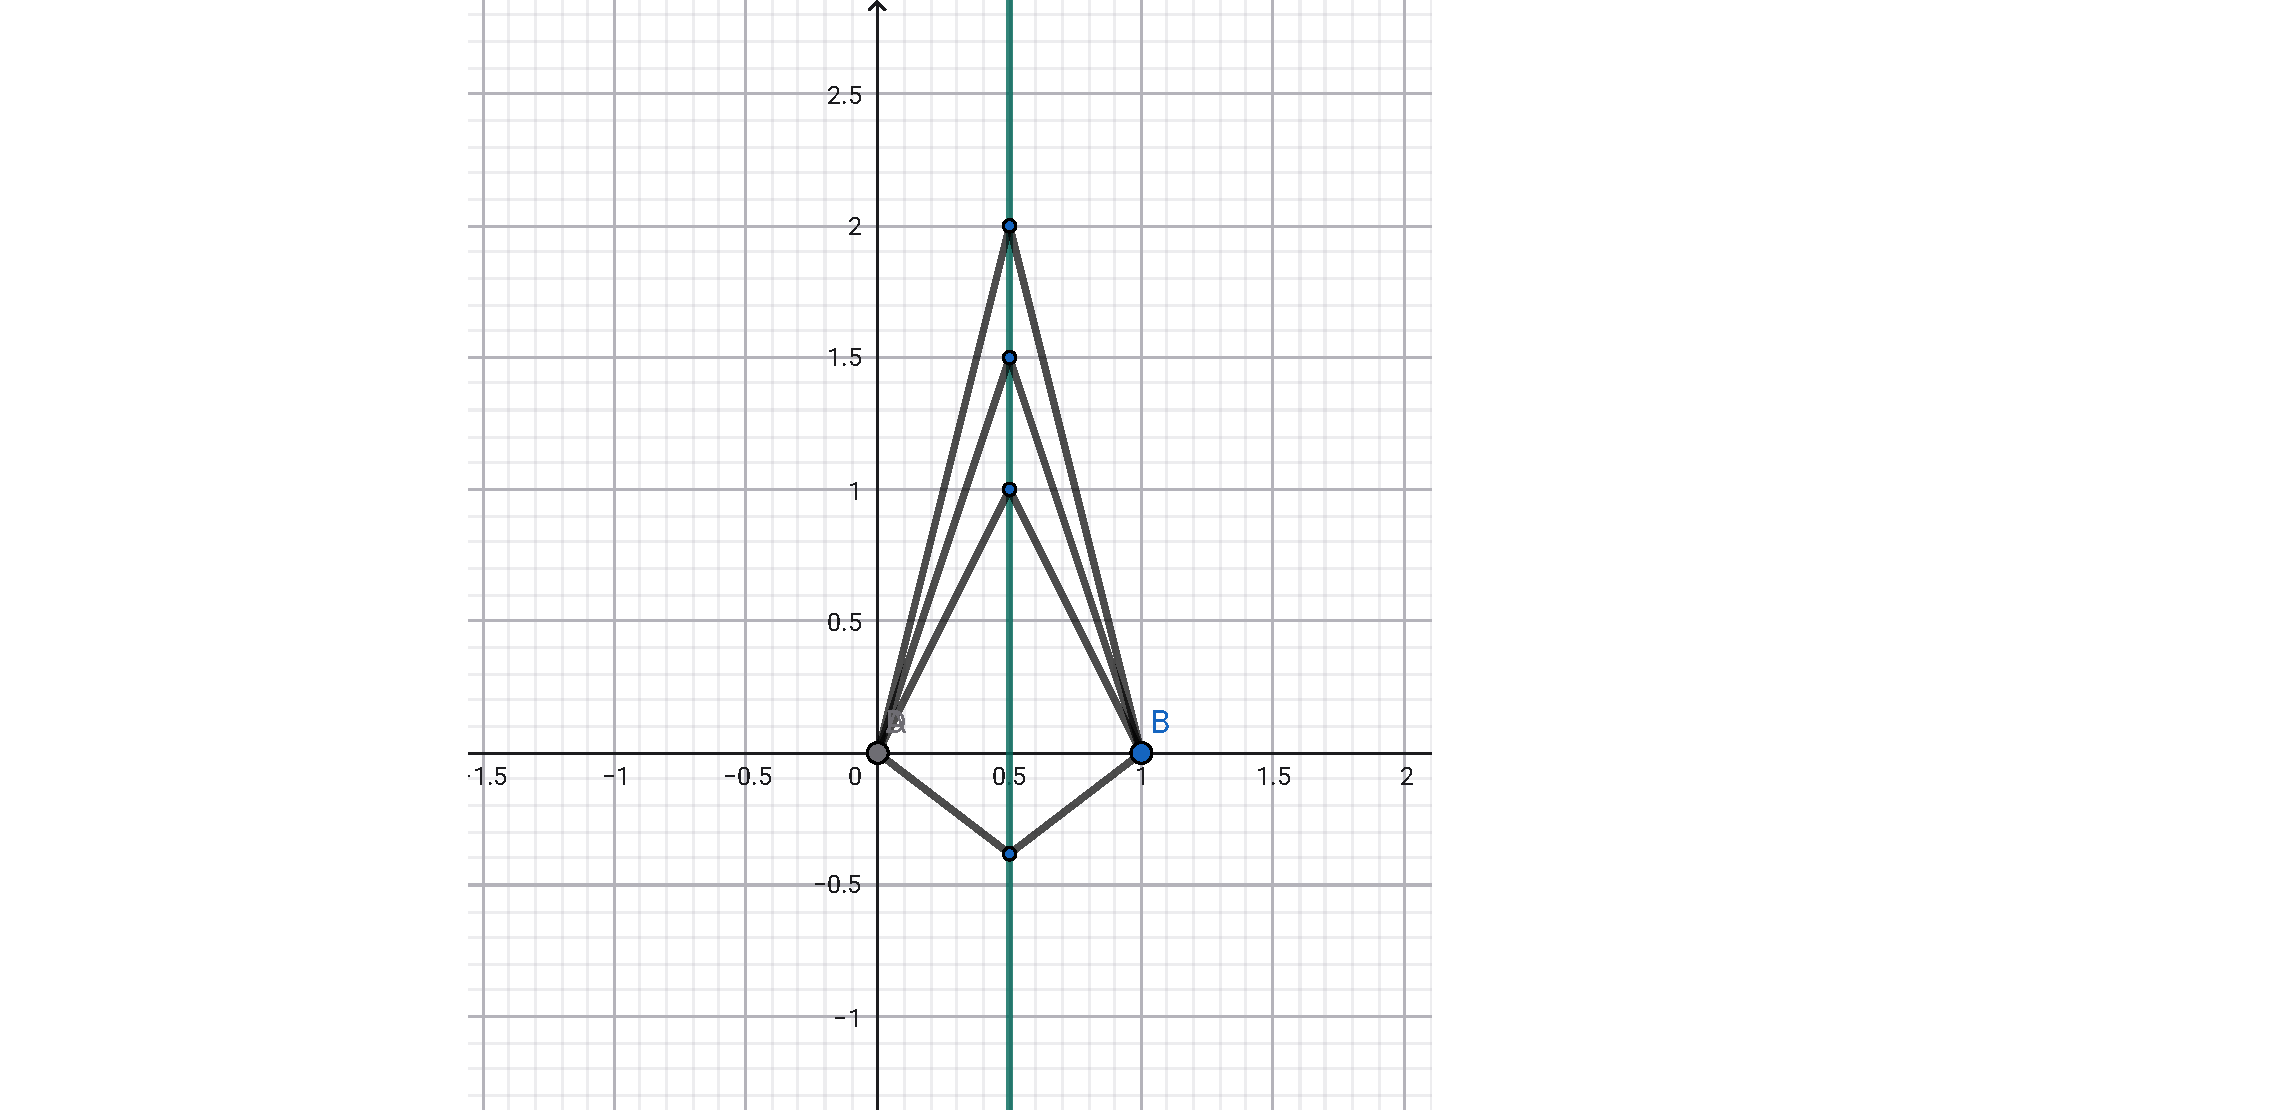
\includegraphics[width=0.6\textwidth]{papers/moebius/bild2.pdf}
	\caption{Nach der Transformation (erstellt mit GeoGebra)}
	
\end{figure}
